\ifdefined\USERMANUAL
  \newcommand{\doctype}{USER'S MANUAL}
\else
  \newcommand{\doctype}{REFERENCE  CARDS}
\fi

\maketitlepage{TAIPO}{MIDI Extender}{TAIPO_SILVER_cutout_small_2}{\doctype}

\newpage
\tableofcontents
\newpage
\part{Overview}
\newpage
\section{Overview}\label{section:installation}
\subsection{Overview}
\paragraph*{}
\textbf{TAIPO} MIDI Extender for The Centre allows connecting The Centre
to the external gear (including computer) via standard MIDI TRS Type B cable.
\subsection{What's in the box}
\paragraph*{}\textbf{TAIPO} comes with standard acessories. Inside box you will find:
\begin{enumerate}
  \item \textbf{TAIPO} Eurorack module
  \item Standard Eurorack power cable (10-pin to 16-pin)
  \item MIDI-EX link cable for linking with \textbf{THE CENTRE}
\end{enumerate}

\newpage
\part{Installation}
\newpage
\section{Installation}
\subsection{Installation steps}
\paragraph*{}
Installing TAIPO follows steps of installing any Eurorack module in the owner's case.

\begin{figure}[h]
  \centering
  \includegraphics[height=0.5\linewidth]{taipo_the_centre_cable_install.jpg}
  \includegraphics[height=0.5\linewidth]{taipo_cable_install.jpg}
  \caption{Cable installation on both ends}
  \label{fig:midsinglenote}
\end{figure}

\subsection{Important installation notes}
\paragraph*{}
 Please note order of colours on both sides. The Centre side colour order from top should be \textbf{BLACK, RED, YELLOW, GREEN} and on the TAIPO side opposite: \textbf{GREEN, YELLOW, RED, BLACK}
\newline$\blacksquare$ IMPORTANT: On The Centre side connect to MIDI-EX connector as depicted on picture above. The second connector is for connecting The Centre's output MIDI to TWINS.

% file format contains all definitions of a patch, connected modules, inputs, outputs and settings. This is the basic binary format of data in The Centre and his completely tied with definition of modules. 
% See: \underline{\nameref{section:oppatch}}

\newpage
\part{MIDI}
\newpage
\section{MIDI Cable Types}
\subsection{TAIPO Cable Type}
\paragraph*{}
TAIPO uses MIDI 3.5mm TRS (Tip-Ring-Shield) Cable Type B See: \underline{\nameref{section:cabletypeb}}
\subsection{About MIDI Signal}
\paragraph*{}
MIDI Signal is send over MIDI Cable using standard RS232 protocol however using 
nonstandard speed of 31250 baud (bits per second). MIDI electrical connection is 
directional meaning that internal connection of pins in cable does matter as the current
flows in one direction. While this is not a problem for standard MIDI DIN type cables 
it became problematic for 3.5mm jack (TRS) based cables as manufacturers started wiring
them differently because no standard has been defined. Based on those wirings a few
standards have emerged.
\newline$\blacksquare$ Different TRS standards are not interchangeable and not compatible. 
To connect defices with different TRS standard a matching cable must be used.
\subsection{DIN Connector}
Standard MIDI cable using 5-pin DIN connector
\subsection{TRS Connector Types}
\subsubsection{Type A Connector}
TRS Type A defines \textbf{TIP} of 3.5mm jack as \textit{\textbf{source}} and \textbf{RING} as \textit{\textbf{sink}}
\newline
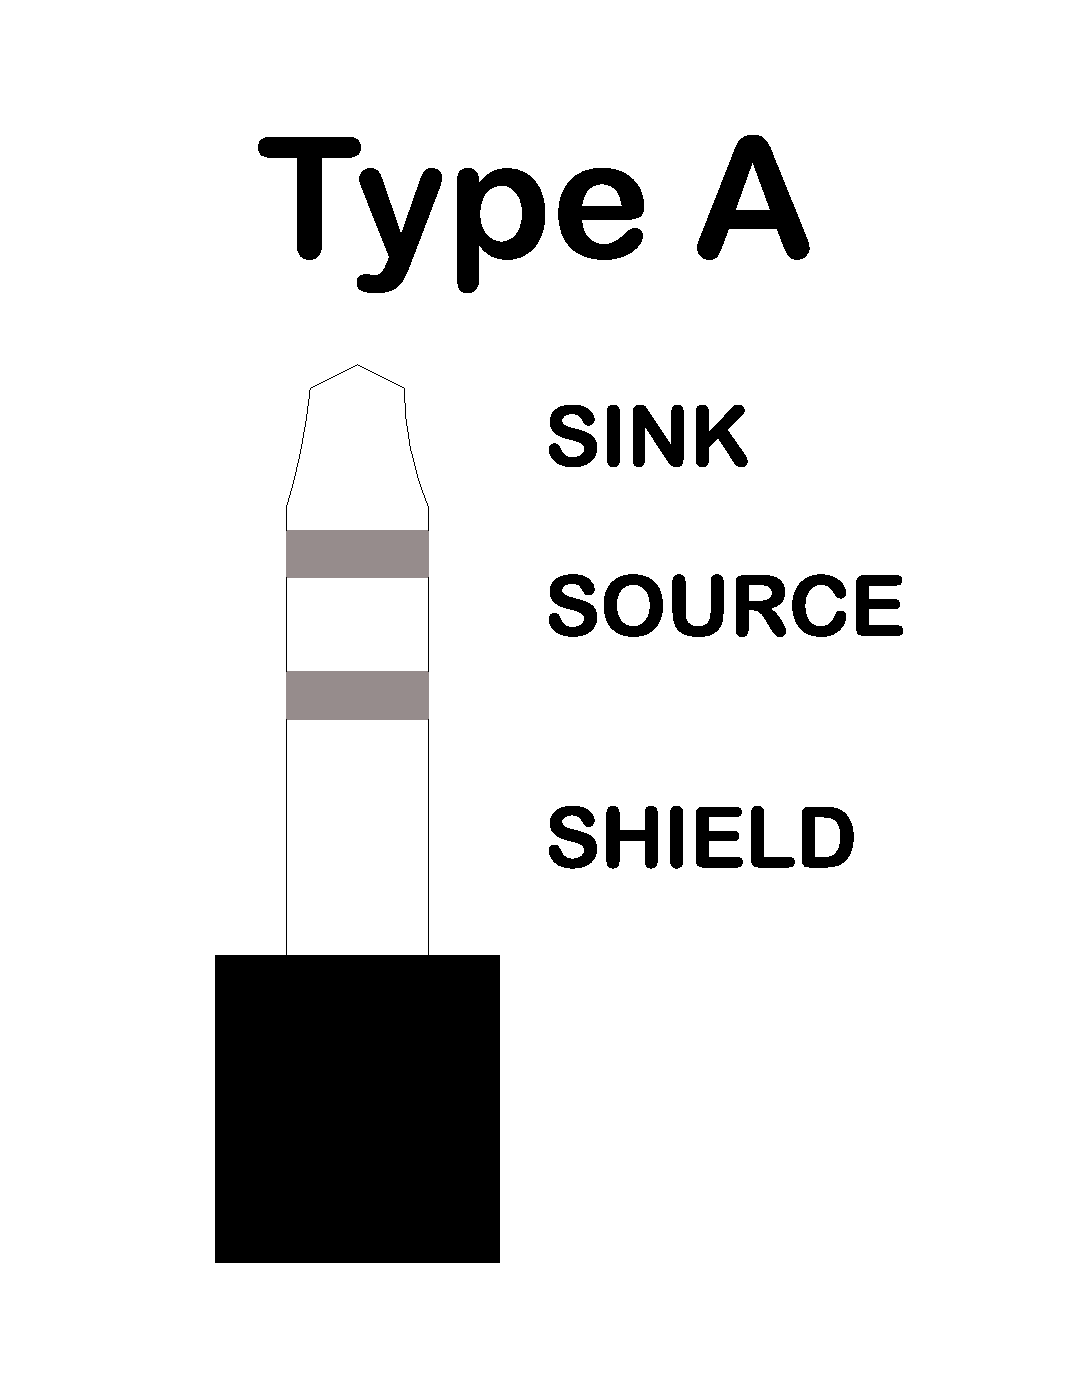
\includegraphics[height=0.3\linewidth]{midi_trs_type_a.eps}
\newline$\bigstar$ Brands that use Type A: Korg, Akai
\subsubsection{Type B Connector}\label{section:cabletypeb}
TRS Type B defines \textbf{TIP} of 3.5mm jack as \textit{\textbf{sink}} and \textbf{RING} as \textit{\textbf{source}}
\newline$\blacksquare$ Type B is more popular among Eurorack Modular scene
\newline
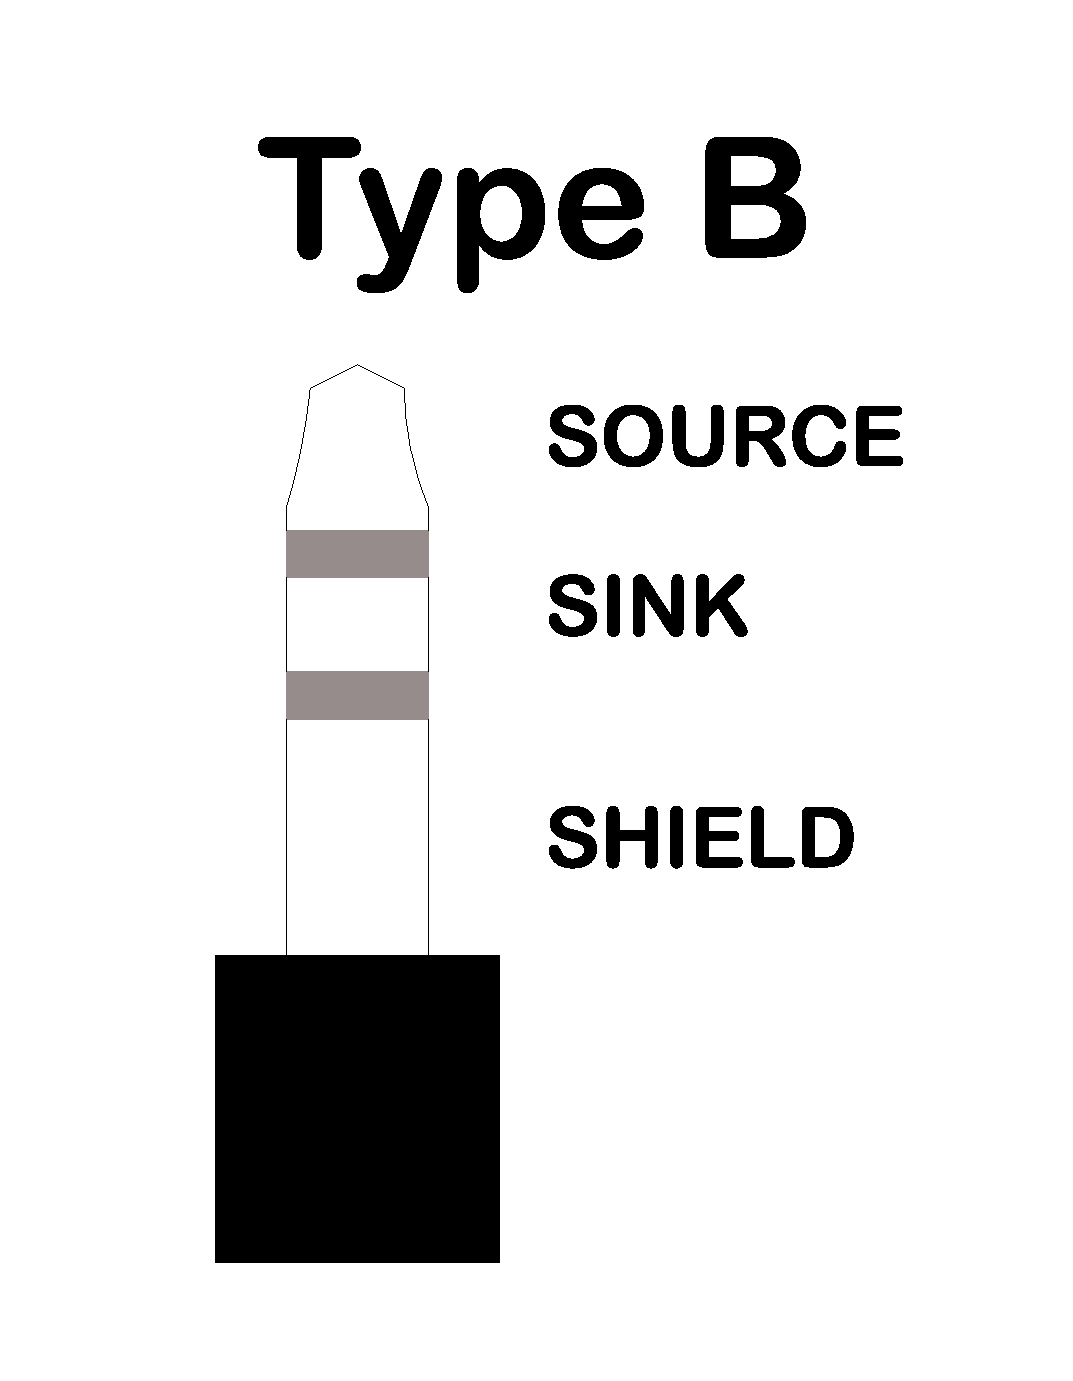
\includegraphics[height=0.3\linewidth]{midi_trs_type_b.eps}
\newline$\bigstar$ Brands that use Type B: Arturia, Novation, 1010
